\documentclass[aspectratio=1610]{beamer}
\usepackage[utf8]{inputenc}
\usepackage{multicol}
\usepackage[czech]{babel}
\usepackage{amsmath}
\usepackage{csquotes}
\usepackage{bold-extra}
\usepackage{listings}

\title{Základy HTML}
\date{WBA | 6. hodina}
\author[Cajthaml]{Matěj Cajthaml}

\usetheme{material}

\usePrimaryCustom

\begin{document}

\begin{frame}
\titlepage
\end{frame}

\begin{frame}{Obsah prezentace}
    \begin{cardTiny}
        \begin{minipage}{\textwidth}
            \vspace{1ex}
            \tableofcontents
        \end{minipage}
    \end{cardTiny}
\end{frame}



\section{Vývojové prostředí kodéra}

\begin{frameImg}[width]{img/computer.jpg}
    \vspace*{60mm}
    \begin{cardTiny}
        \vspace*{\fill}
        \begin{center}
            \textbf{Vývojové prostředí}
        \end{center}
    \end{cardTiny}
\end{frameImg}

\begin{frame}{Vývojové prostředí}
    \begin{cardTiny}
        \begin{flushleft}
            Program ve kterém se píše kód.

            Často nemusí být ani program - jen webová stránka.

            Pomáhá (napovídáním, označením chyb) koderovi psát kód.

            Kompiluje či spouští kód.
        \end{flushleft}
    \end{cardTiny}
\end{frame}

\begin{frame}
    \begin{center}
        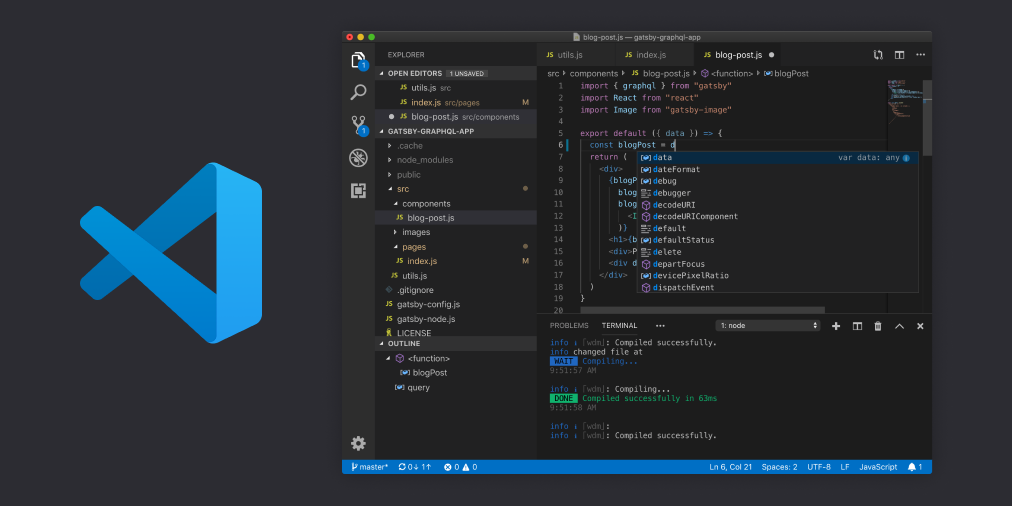
\includegraphics[width=\textwidth]{img/vscode.png}
    \end{center}
\end{frame}

\begin{frame}{Vývojové prostředí ve škole}
    \begin{cardTiny}
        \begin{flushleft}
            VSCode

            \vspace{3ex}
            Notepad++

            \vspace{3ex}
            Brackets

            \vspace{3ex}
            PSPad

            \vspace{3ex}
            Nebo online služby (w3schools.com, codesandbox.io, codepen.io).
        \end{flushleft}
    \end{cardTiny}
\end{frame}

\begin{frame}{Vývojové prostředí ve škole}
    \begin{cardTiny}
        \begin{center}
            \textbf{ÚKOL}
        \end{center}
        \begin{flushleft}
            Vyberte si z některých vývojových prostředí (VSCode, Backets, online služby, ...). S tímto vývojovým prostředím se naučte pracovat (vytvářet složky, soubory, ...). Popř. se podívejte na online návody.
            
            \vspace{2ex}
            Vytvořte si osobní místo na svém disku, kde budete uchovávat svoje zdrojové kódy.
        \end{flushleft}
    \end{cardTiny}
\end{frame}



\section{HTML}

\begin{frameImg}[width]{img/html.jpg}
    \vspace*{60mm}
    \begin{cardTiny}
        \vspace*{\fill}
        \begin{center}
            \textbf{HTML}
        \end{center}
    \end{cardTiny}
\end{frameImg}

\begin{frame}{HTML}
    \begin{cardTiny}
        = \textbf{Hyper Text Markup Language}.

        Tzv. značkovací jazyk (pomocí tagů).

        HTML dokument obsahuje tagy a text.

        \vspace{2ex}

        1990 - vzniklo HTML.

        2012 - vzniklo HTML5.
    \end{cardTiny}
\end{frame}

\begin{frame}{Soubory webových stránek}
    \begin{multicols}{2}
        \centering
        \begin{cardTiny}
            \textbf{HTML}

            \begin{flushleft}
            Samotné soubory, obsahující tagy - definici webových stránek. 

            Používají příponu \texttt{.html}.
            \end{flushleft}
        \end{cardTiny}
        \begin{cardTiny}
            \textbf{Obrázky}


            \begin{flushleft}
            Soubory obsahující obrázky.

            Vektorové obrázky.

            Používají se přípony \texttt{.jpg}, \texttt{.png}, \texttt{.gif},  \texttt{.svg}.
            \end{flushleft}
        \end{cardTiny}
        \begin{cardTiny}
            \textbf{Index}

            \begin{flushleft}

            Speciální soubor nazývaný \texttt{index}.

            Při přístupu do složky se zobrazí právě daný soubor.

            Obvykle \texttt{index.html}. 
            \end{flushleft}
        \end{cardTiny}
        \begin{cardTiny}
            \textbf{Všechny soubory}


            \begin{flushleft}
            Bez diakritiky, bez mezer, malé písmena, malé délky.
            \end{flushleft}
        \end{cardTiny}
    \end{multicols}
\end{frame}



\section{Tagy}
\begin{frame}{Tag}
    \begin{cardTiny}
        Tag je značka HTML určující určitý typ obsahu.

        Vždy se zapisuje v špičatých závorkách (\texttt{< a >}).

        Každý tag má svojí určitou funkčnost.

        Malé písmena (velké jsou však platná).
    \end{cardTiny}
    \begin{cardTiny}
        \begin{center}
        \textbf{Párový tag}

        Pozice vymezuje odkud kam platí.

        \texttt{tady neplatí <tag>\textbf{tady platí}</tag> a tady už ne}
        \end{center}
    \end{cardTiny}
    \begin{cardTiny}
        \begin{center}
        \textbf{Nepárový tag}

        \texttt{dobrý <tag> den} == \texttt{dobrý <tag/> den}
        \end{center}
    \end{cardTiny}
\end{frame}

\begin{frame}{Ukázkové tagy}
    \begin{cardTiny}
        \begin{center}
        \textbf{Párové tagy}

        a, p, b, u, i
        \end{center}
    \end{cardTiny}
    \begin{cardTiny}
        \begin{center}
        \textbf{Nepárové tagy}

        br, img, hr, link
        \end{center}
    \end{cardTiny}
\end{frame}

\begin{frame}{Křížení tagů}
    \begin{cardTiny}
        \begin{center}
        \textbf{VALIDNÍ}

        \texttt{<p>test<i>ovací</i> text</p>}
        \end{center}
    \end{cardTiny}
    \begin{cardTiny}
        \begin{center}
        \textbf{NENÍ VALIDNÍ}

        \texttt{<p>test<i>ovací</p> text</i>}
        \end{center}
    \end{cardTiny}
\end{frame}



\section{Elementy}
\begin{frame}{Element}
    \begin{cardTiny}
        Element je kompletní celek.

        Obsahuje počáteční tag, obsah a ukončující tag.

        Pouze párové tagy!
    \end{cardTiny}
    \begin{cardTiny}
        \begin{itemize}
        \item \texttt{<b>}
        \item \texttt{Tlustý text!}
        \item \texttt{</b>}
        \end{itemize}
    \end{cardTiny}
\end{frame}



\section{Atributy}
\begin{frame}{Atribut}
    \begin{cardTiny}
        Každý tag může mít nekonečně mnoho \textbf{atributů}.

        Každý tag má své atributy, které na něm fungují. 

        Každý atribut má svojí hodnotu.

        Atribut určuje určitou vlastnost nebo chování daného tagu a jeho dětí.
    \end{cardTiny}
    \begin{cardTiny}
        \begin{center}
        \texttt{\textbf{<tag atribut=''hodnota''>text</tag>}}
        \end{center}
    \end{cardTiny}
\end{frame}

\begin{frame}{Odkaz}
    \begin{cardTiny}
        \begin{center}
        \texttt{\textbf{<a href=''https://google.com''>odkaz na google</a>}}
        \end{center}
    \end{cardTiny}
\end{frame}

\begin{frame}{Nejpoužívanější atributy}
    \begin{cardTiny}
        \begin{flushleft}
            Nejpoužívanější atributy na webových stránkách jsou \texttt{id} a \texttt{class}.

            \vspace{3ex}
            id (identifikátor) - určuje \textbf{JEDEN tag} na celé stránce.

            \vspace{2ex}
            class (třída) - určuje třídy, může být přiřazené více prvkům. 
        \end{flushleft}
    \end{cardTiny}
\end{frame}



\section{HTML komentáře}
\begin{frame}{HTML komentáře}
    \begin{cardTiny}
        \begin{center}
        \texttt{<!--} komentář \texttt{-->}
        \end{center}
    \end{cardTiny}
\end{frame}



\section{Struktura HTML}
\begin{frame}{Struktura HTML}
    \begin{cardTiny}
        \begin{flushleft}
            Každá stránka by měla mít tyto základní elementy.
        \end{flushleft}
    \end{cardTiny}
    \begin{cardTiny}
        \begin{flushleft}
            DOCTYPE

            HTML

            HEAD

            TITLE

            BODY
        \end{flushleft}
    \end{cardTiny}
\end{frame}

\begin{frame}{Základní struktura - DOCTYPE}
    \begin{cardTiny}
        \begin{flushleft}
            Určuje verzi HTML, ve které se webová stránka má vykreslit.

            Používáme pouze definici pro HTML5.
        \end{flushleft}
    \end{cardTiny}
    \begin{cardTiny}
        \begin{flushleft}
        \texttt{\textbf{<!DOCTYPE html>}}
        \end{flushleft}
    \end{cardTiny}
\end{frame}

\begin{frame}{Základní struktura - HTML}
    \begin{cardTiny}
        \begin{flushleft}
            Ohraničení celého kódu webové stránky.

            Určuje kde začínají a končí příkazy HTML.
        
            Pomocí atributu lang určuje jazyk stránky.
        \end{flushleft}
    \end{cardTiny}
    \begin{cardTiny}
        \begin{flushleft}
        \texttt{\textbf{<!DOCTYPE html><html>...</html>}}
        \end{flushleft}
    \end{cardTiny}
\end{frame}

\begin{frame}{Základní struktura - HEAD}
    \begin{cardTiny}
        \begin{flushleft}
            Obsahuje definice stránky, které určují její vzhled a chování.

            \textbf{Neobsahuje vše, co se NEvykresluje v prohlížeči.}

            Nadpis stránky, styly, ...
        \end{flushleft}
    \end{cardTiny}
    \begin{cardTiny}
        \begin{flushleft}
        \texttt{\textbf{<!DOCTYPE html><html><head>...</head>...</html>}}
        \end{flushleft}
    \end{cardTiny}
\end{frame}

\begin{frame}{Základní struktura - TITLE}
    \begin{cardTiny}
        \begin{flushleft}
            Pouze v hlavičce - HEAD.

            Uvádí titulek stránky, který se zobrazuje v kartě.
        \end{flushleft}
    \end{cardTiny}
    \begin{cardTiny}
        \begin{flushleft}
        \texttt{\textbf{<!DOCTYPE html><html><head><title>Smíchovská střední průmyslová škola</title></head>...</html>}}
        \end{flushleft}
    \end{cardTiny}
\end{frame}

\begin{frame}
    \begin{center}
        
\includegraphics[width=\textwidth]{img/tab-ssps.png}
    \end{center}
\end{frame}

\begin{frame}{Základní struktura - META}
    \begin{cardTiny}
        \begin{flushleft}
        Určuje např. kódování textu, velikost.
        \end{flushleft}
    \end{cardTiny}
    \begin{cardTiny}
        \begin{flushleft}
        \texttt{\textbf{<meta charset=''UTF-8''>}}
        
        \texttt{\textbf{<meta name=''viewport'' content=''width=device-width, initial-scale=1.0''>}}
        \end{flushleft}
    \end{cardTiny}
\end{frame}

\begin{frame}{Základní struktura - BODY}
    \begin{cardTiny}
        \begin{flushleft}
            Obsahuje vše, co se vykresluje na stránce.
        \end{flushleft}
    \end{cardTiny}
    \begin{cardTiny}
        \begin{flushleft}
        \texttt{\textbf{<!DOCTYPE html><html><head><title>Smíchovská střední průmyslová škola</title></head><body>...</body></html>}}
        \end{flushleft}
    \end{cardTiny}
\end{frame}

\begin{frame}{Základní struktura}
    \begin{center}
        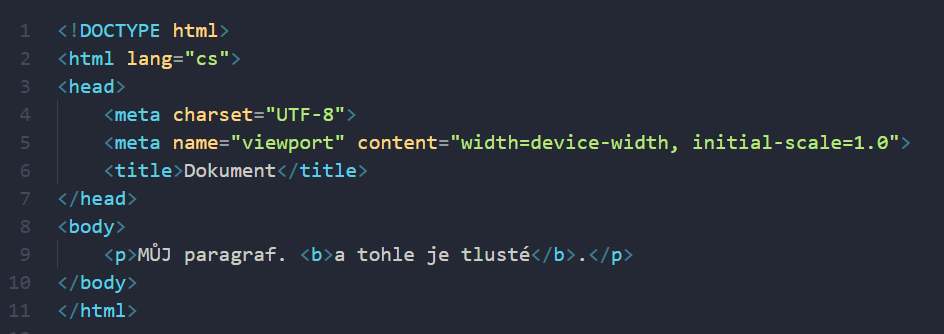
\includegraphics[width=\textwidth]{img/html-6.png}
    \end{center}
\end{frame}

\begin{frame}{Základní struktura}
    \begin{center}
        
\includegraphics[width=\textwidth]{img/html-6-render.png}
    \end{center}
\end{frame}



\section{HTML entity}
\begin{frame}{HTML entita}
    \begin{cardTiny}
        \begin{flushleft}
            Zkratka pro znaky, které se těžko v prohlížeči zobrazují.

            Jedná se například o \texttt{< a >}.

            Základní seznam \href{https://www.w3schools.com/html/html_entities.asp}{ODKAZ}.
        \end{flushleft}
    \end{cardTiny}
    \begin{cardTiny}
        \begin{center}
        \texttt{\&kódznaku;}

        \texttt{\&\#číslo;}
        \end{center}
    \end{cardTiny}
    \begin{cardTiny}
        \begin{center}
        \texttt{\&copy;} $\rightarrow$ \texttt{©}
        \end{center}
    \end{cardTiny}
\end{frame}



\section{Vývojové prostředí kodéra doma}

\begin{frame}{Vývojové prostředí doma}
    \begin{cardTiny}
        \begin{center}
            \textbf{POVINNÝ DOMÁCÍ ÚKOL}
        \end{center}
        \begin{flushleft}
            Nainstalujte si nějaké vývojové prostředí do počítače doma / do notebooku. Naučte se s vývojovým prostředím pracovat, jak vytvářet soubory a upravovat je.

            \vspace{2ex}
            Vytvořte HTML soubor s ukázkovou strukturou a zobrazte jej v prohlížeči. Vyscreenshotujte celou obrazovku s vývojovým prostředím a prohlížečem a odešlete jej na e-mail matej.cajthaml@ssps.cz. 
            
            \vspace{2ex}
            Viz. \textbf{\href{https://cajthaml.eu/predmet/wba/ukol/vyvojove-prostredi}{https://cajthaml.eu/predmet/wba/ukol/vyvojove-prostredi}}

            Termín: 29. 9. 2020 do 18:00 (po 22:00 již -2 body)

            \vspace{2ex}
            Bodový základ: 3 body.

            Úspěšné splnění +3 body, pozdě: -1 bod za každou započatou hodinu, nesplnění max. -2 body. 
        \end{flushleft}
    \end{cardTiny}
\end{frame}



\section{Shrnutí}
\begin{frame}{Shrnutí 1}
    \begin{cardTiny}
        \begin{center}
            \textbf{Co je to HTML entita?}
        \end{center}
    \end{cardTiny}
    \begin{cardTiny}
        \begin{center}
            \textbf{Proč se nesmí křížit tagy?}
        \end{center}
    \end{cardTiny}
    \begin{cardTiny}
        \begin{center}
            \textbf{Jaký je rozdíl mezi tagem a elementem?}
        \end{center}
    \end{cardTiny}
    \begin{cardTiny}
        \begin{center}
            \textbf{Jaký je rozdíl mezi identifikátorem a třídou?}
        \end{center}
    \end{cardTiny}
    \begin{cardTiny}
        \begin{center}
            \textbf{Jakým tagem se určuje nadpis stránky?}
        \end{center}
    \end{cardTiny}
\end{frame}

\begin{frame}{Shrnutí 2}
    \begin{cardTiny}
        \begin{center}
            \textbf{Jaké části struktury musí webová stránka vždy obsahovat?}
        \end{center}
    \end{cardTiny}
    \begin{cardTiny}
        \begin{center}
            \textbf{Co je to vývojové prostředí?}
        \end{center}
    \end{cardTiny}
    \begin{cardTiny}
        \begin{center}
            \textbf{Co je to soubor index?}
        \end{center}
    \end{cardTiny}
    \begin{cardTiny}
        \begin{center}
            \textbf{Jaký je rozdíl mezi vektorovým a obyčejným obrázkem?}
        \end{center}
    \end{cardTiny}
    \begin{cardTiny}
        \begin{center}
            \textbf{Jakým tagem se určuje tlusté písmo?}
        \end{center}
    \end{cardTiny}
\end{frame}

\end{document}